\documentclass[11pt, letterpaper]{article}
\usepackage[margin=0.5in]{geometry}
\usepackage{graphicx}

\begin{document}

\title{String Search}
\author{Audrey Weaver}
\maketitle

\section{Introduction}
An organism's DNA encompasses all instructions for its development and
function. To link specific DNA sequences to particular traits or diseases, we
analyze the DNA of individuals exhibiting similar or differing characteristics.
DNA's structure—a long sequence of nucleotides denoted by A, C, T, and
G—transforms the comparison of two genomes into a computational string search
challenge. This problem involves two input strings: a typically longer string,
the text $T$, and a usually shorter string, the pattern $P$. The
objective is to locate every instance of $P$ within $T$. Here we analyze the
the efficiency and memory consumption of a basic string search algorithm, 
naive search, and a more advanced string search algorithm, Boyer Moore, that
aligns $P$ with all possible positions in $T$.  The naive search algorithm's
runtimes correlated with $T$'s length and additional memory requirement were
minimal. The Boyer Moore algorithm required a more memory consistently across
experimentation. 

\section{Results}

As expected, the runtime of the naive string search algorithm increased
linearly and the memory usage remained constant as the text size increased
(Figure~\ref{timeandmem}). The algorithm's runtime increased linearly with
the text size because the algorithm considers all possible alignments of the
pattern $P$ with the text $T$. As the text size increases, the number of
possible alignments increases linearly. The algorithm's memory usage remained
constant because the algorithm only stores the positions of the pattern $P$ in
the text $T$.


\begin{figure}[ht] \centering
    \includegraphics[width=0.6\textwidth]{./doc/naive_search.png}
    \caption{The empirical runtime and memory usage of the naive string search
    algorithm considering a pattern size of 100 and a database size ranging
    from 100 to 10,000 characters.}
    \label{timeandmem}
\end{figure}

Niether the runtime nor the memory usage of the Boyer Moore algorithm varied 
significantly during the experiment. This is to be expected as the Boyer Moore 
algorithm uses heuristics, the bad character table, and the good suffix table 
to determine skip length and avoid comparing every character. Because of its
speed, the Boyer Moore model is more efficient overall especially on larger 
sequences or situations where $P$ is rare in $T$. The memory usage is 
consistently higher in the Boyer Moore model as it requires storage of the 
good suffix table and the bad character table. 

\begin{figure}[ht] \centering
    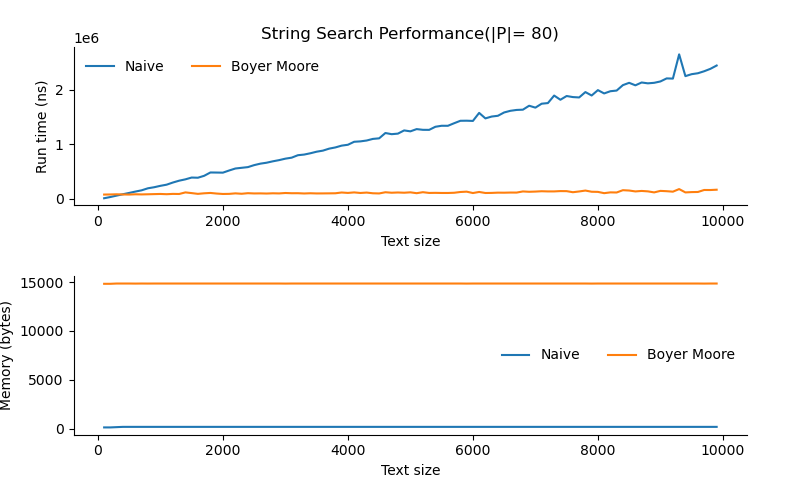
\includegraphics[width=0.6\textwidth]{./doc/results10000.png}
    \caption{The empirical runtime and memory usage of the naive string search
    algorithm and the Boyer Moore search algorithm considering a pattern size 
    of 80 and a database size ranging from 100 to 10,000 characters.}
    \label{timeandmem}
\end{figure}

\section{Methods}

\subsection{Naive string search}
The naive string search algorithm considers all possible alignments of the
pattern $P$ with the text $T$. Staring at the first position in $T$, the
algorithm compares $P$'s characters with the corresponding characters in $T$.
If all characters match, the algorithm records the alignment's position in $T$.
The algorithm then repeats this process for the next alignment. If any of the 
characters in $P$ do not match a corresponding character in $T$, the current
alignment breaks and then $P$ shifts down one position in $T$, and the process
repeats. This process continues until $P$ has been compared to all possible
alignments in $T$, then returns the recorded positions.

\subsection{Boyer Moore string search}
The Boyer Moore search algorithm improves upon the naive search because it 
skips sections of characters where a match is impossible. Therefore, it is 
significantly fasterwith a large or very unique text. Boyer Moore computes 
and stores heuristics: the bad character rule which shifts $P$ based on the 
last occurence of the mismatched character in $P$, and the good suffix rule 
which shifts $P$ when a suffix of $P$ matches $T$. The algorithm compares $P$ 
to $T$ from right to left, using the stores heuristics to determine the shift 
length before continuing to search. This process continues until P has been 
compared to all possible allignments in T, then it returns the recorded 
positions where $P$ occurs.

\subsection{Empirical comparison}
We evaluated the performance of the naive string search and Boyer Moore 
algorithms considering a pattern size of 80 and text sizes that ranged 
from 100 to 10,000 characters with a step size of 100.  The performance 
metrics include runtime and memory usage. For each text size, we ran a 
single search where we generated a random string for $T$ from the alphabet 
${A, C, T, G}$ and extracted a random substring $P$ from $T$. We then 
recorded the runtime and memory usage of the algorithm consiuder that $P$ 
and $T$. After ten rounds were complete for a given text size, we calculated 
the average runtime and memory usage for the search.

\subsection{Reproducibility}
To replicate these experiments, clone the repository and then run the
following commands from the root directory of the repository.

\begin{verbatim}
$ git clone https://github.com/cu-compg-spring-2025/assignment-4-string-search-audreyw04.git
$ cd string_search
$ python src/string_search.py \
    --text_range 100 10000 100 \
    --pattern_size 80 \
    --out_file doc/results10000.png

    python ./src/string_search.py --text_range 1000 10000 100 --pattern_size 80 --out_file results10000.png
\end{verbatim}

\end{document}
